\documentclass[11pt,a4paper]{article}

\usepackage[utf8]{inputenc}
\usepackage{amsmath, amssymb, latexsym}

\usepackage[left=2cm,right=2cm,top=2cm,bottom=2cm]{geometry}
\usepackage{tikz}
\usetikzlibrary{decorations.pathreplacing}
\usetikzlibrary{fadings}
\usepackage{lscape}

\begin{document}
\begin{landscape}

\begin{figure}[t!]
	\centering
\begin{tikzpicture}
    \node[anchor=south west,inner sep=0] at (-1,0) {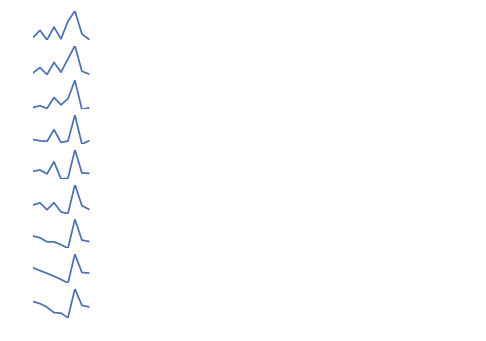
\includegraphics[scale=0.75]{raw1.png}};
    \node at (2,10){\begin{tabular}{c}convolutional layer\\64 filters, subsample=2\\layer $l = 1$\end{tabular}};
     \node[anchor=south west,inner sep=0] at (2,0) {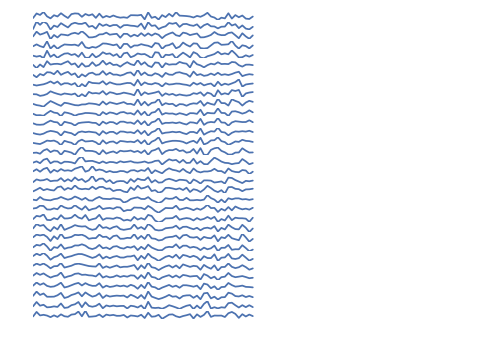
\includegraphics[scale=0.75]{features1.png}};
        \node at (9,10){\begin{tabular}{c}max-pooling layer\\pooling length=64\\layer $l = 2$\end{tabular}};
       \node[anchor=south west,inner sep=0] at (9,0) {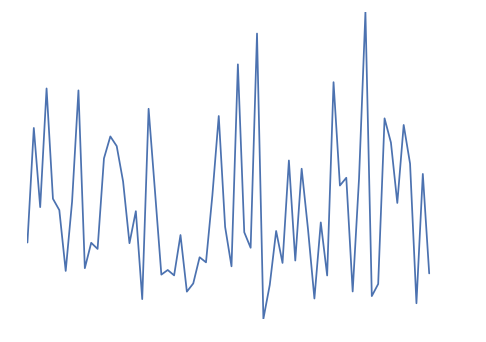
\includegraphics[scale=0.65]{features2.png}};
\end{tikzpicture}
\end{figure}
\end{landscape}
\end{document}